% ------------------------------------------------------------------------------------
%                                CONCETTI GENERALI
% ------------------------------------------------------------------------------------

\chapter{Concetti generali dell'ottimizzazione}

\section{Nozioni paradigma-indipendenti}

La teoria e gli algoritmi sviluppati per affrontare problemi nei quattro paradigmi presentati
sopra sono notevolemente diversi gli uni dagli altri; tuttavia esistono \textbf{alcuni concetti 
fondamentali} che sono \textbf{comuni a tutti gli approcci dell'ottimizzazione}, anche 
\textbf{indipendentemente dal paradigma}. 

\subsection{Inferenza}

In un problema di ottimizzazione, può capitare che un \textbf{vincolo} $C$ sia
\textbf{dedotto} (derivato) da un \textbf{insieme di vincoli} $S$.

\begin{definition}[VINCOLO DEDOTTO]
    Se \textbf{ogni} $x\in D$ che \textbf{soddisfa} $S$ \textbf{soddisfa
    anche} $C$, allora diciamo che $C$ è un \textbf{vincolo dedotto}.
\end{definition}

Chiaramente, dal punto di vista della modellazione, un tale vincolo è \textbf{ridondante}
dato che \textbf{non cambia l'insieme delle soluzioni ammissibili}; tuttavia potrebbe
rivelarsi (in alcuni casi) molto utile per \textbf{l'efficienza degli algoritmi di 
ricerca} in quanto potrebbe \textit{"esplicitare" informazioni} che \textit{non sono
derivabili da nessun altro vincolo se preso singolarmente}.

\begin{exa}
    Consideriamo ad esempio la seguente regione ammissibile:
    \[
        \begin{aligned}
            x_{1} + x_{2} \ge 1 & & x_{1}-x_{2} \ge 0 & & x_{1},x_{2} \in \{0,1\}  
        \end{aligned}
    \]
    E' immediato verificare che $x_{1}=1$ è un \textbf{vincolo valido} per $S$, ma
    \textbf{non è immediatamente deducibile} dai due vincoli sopra se 
    \textbf{presi separatamente}.
\end{exa}

\subsection{Ricerca}

Un concetto molto importante è quello di ricerca:

\begin{definition}[RICERCA]
    Dato un problema $P$, la \textbf{ricerca} consiste nel \textbf{risolvere una serie di
    restrizioni} 
    \[
        P_{1}, \ldots , P_m 
    \] 
    di $P$.

    Le \textbf{restrizioni} sono \textbf{ottenute aggiungendo dei vincoli} al
    problema originale.
\end{definition}

In altre parole, rendiamo \textit{più "stringente"} il problema andando ad aggiungere
ulteriori vincoli. L'intuizione alla base delle restrizioni è che in alcuni casi
potrebbe risultare \textit{conveniente} aggiungere dei vincoli per \textbf{restringere 
lo spazio delle soluzioni}, in modo tale da rendere il problema \textbf{più
facile da risolvere}.

In particolare, sono importanti le \textbf{ricerche esaustive}:

\begin{definition}[RICERCA ESAUSTIVA]
    Una ricerca si dice \textbf{esaustiva} se l'insieme delle restrizioni considerate
    \textbf{"copre" tutto lo spazio} delle \textbf{soluzioni ammissibili} di $P$:
    \[
        \bigcup_i F(P_i) = F(P)
    \] 
\end{definition}

Nel caso di una ricerca esaustiva, possiamo \textbf{rivolvere} $P$ \textbf{risolvendo
tutte le restrizioni} $P_i$ e \textbf{scegliendo la soluzione migliore}.

In ogni caso, è importante il seguente fatto:

\begin{prop}
    Data una restrizione $P_i$, una \textbf{sua qualsiasi soluzione
    ammissibile} è \textbf{ammissibile anche} per il problema di partenza $P$.

    In particolare se $\tilde{x}$ è \textbf{soluzione ottima della restrizione}, essa
    rappresenta un \textbf{upper bound} per la \textbf{soluzione al problema 
    originale} $x^{*}$:
    \[
        x^* \le \tilde{x}
    \] 
\end{prop}

L'intuizione dietro al fatto è la seguente:

\begin{remark}[INTUIZIONE]
    Le soluzioni di $P_i$ sono un \textbf{sottoinsieme delle soluzioni originali},
    per cui una soluzione di $P_i$ deve \textbf{essere anche soluzione} di $P$.

    Inoltre, se $\tilde{x}$ è \textbf{soluzione ottima della restrizione}, sappiamo
    che la \textbf{soluzione al problema originale} sarà \textbf{"almeno così
    tanto buona"}.
\end{remark}

\subsection{Rilassamento}

Il \textit{rilassamento} è il concetto complementare alla restrizione. Un 
rilassamento $R$ è ottenuto da un problema di ottimizzazione $P$:
\begin{enumerate}
    \item Eliminando alcuni vincoli.
    \item Sostituendo la funzione obiettivo $f(x)$ con la sua \textit{approssimazione
        inferiore} $g(x)$.
\end{enumerate}

Più formalmente:

\begin{definition}[RILASSAMENTO]
    $R$ è un \textbf{rilassamento} di $P$ se:
    \begin{enumerate}
        \item $F(P) \subseteq F(R)$
        \item $g(x)\le f(x)$  $\forall x\in F(P)$
    \end{enumerate}
\end{definition}

In maniera analoga a quanto detto per le restrizioni, l'idea è che a volte 
potrebbe risultare più semplice risolvere una \textit{"versione rilassata"} del
problema.

\begin{warn}
    Sebbene si possano ricavare informazioni utili, bisogna fare attenzione 
    al fatto che il \textbf{problema NON è equivalente}.
\end{warn}

In tal senso, è utile considerare le seguenti proposizioni:

\begin{prop}
    Dato un problema $P$ ed un suo rilassamento $R$ è possibile derivare che:
    \begin{enumerate}
        \item Se $F(R)=\emptyset$, allora $P$ è \textbf{impossibile}.
        \item Se $x^*$ è \textbf{soluzione ottima} di $R$, $g(x^*)$ è un \textbf{lower
            bound} per il \textbf{valore ottimo} di $P$.
        \item Se $x^*$ è \textbf{soluzione ottima} di $R$, $x^*\in F(P)$ e
            $g(x^*)=f(x^*)$, allora $x^*$ è \textbf{ottima} per $P$.
    \end{enumerate}
\end{prop}

E' utile discutere i tre punti:

\begin{remark} Possiamo intuire che:
    \begin{enumerate}
        \item Se il \textbf{rilassamento} (la versione "semplificata") 
            è \textbf{impossibile}, lo \textbf{deve essere anche
            il problema originale}.
        \item La soluzione ottima del rilassamento ci fornisce un
            \textbf{"tetto massimo"} per la \textbf{"bontà" della soluzione}: avendo
            "accesso" solo ad un sottoinsieme delle soluzioni, quella di nostro
            interesse sicuramente \textit{non potrà essere migliore}.
        \item Si tratta di un \textbf{caso fortunato}: se la soluzione del rilassamento
            è \textbf{ottima}, \textbf{ammisibile} per $P$, e i \textbf{valori delle
            funzioni obiettivo coincidono}, allora $x^*$ è \textbf{ottima anche per} $P$.
    \end{enumerate}
\end{remark}

\subsection{Dualità}

Un problema di ottimizzazione $P$ viene spesso \textbf{interpretato come problema di 
ricerca} (problema \textit{primario}): vogliamo \textbf{"cercare" la soluzione ottima}.

Alternativamente, lo stesso problema può anche essere visto come un \textbf{problema
di inferenza} (problema \textit{duale}): a partire dai vincoli, vogliamo \textbf{derivare il più stretto
lower bound possibile} su $f(x)$.

\begin{definition}[PROBLEMA DUALE]
    Il problema di \textbf{trovare la dimostrazione} che \textbf{porta al
    lower bound più stretto} prende il nome di \textbf{problema duale}.
\end{definition}

\begin{remark}[INTERPRETAZIONE]
    In altre parole:
    \begin{itemize}
        \item Il problema \textbf{originale} cerca di \textbf{"scendere" verso il valore minimo} 
        trovando \textbf{soluzioni ammissibili via via migliori}, 
        \item Il problema \textbf{duale} cerca di \textbf{"salire"} costruendo un 
        \textbf{limite inferiore sempre più alto}, manipolando i vincoli a disposizione. 
    \end{itemize}
\end{remark}

Questo è un punto cardine della programmazione matematica, dato che permette di 
\textbf{certificare l'ottimalità di una soluzione}: quando il \textbf{valore ottenuto dalla ricerca} 
coincide con il \textbf{limite inferiore dimostrato dall'inferenza}, si ha la \textbf{garanzia} di aver 
trovato l'\textbf{ottimo globale}.

\section{Approcci di ricerca}

\subsection{Ricerca naive: Generate-And-Test}

Un possibile approccio per applicare la ricerca ad un problema di ottimizzazione
è \textit{generate-and-test}. Banalmente, l'idea di base è la seguente:

\begin{definition}[GENERATE-AND-TEST]
    Generiamo \textbf{tutte le soluzioni} possibili, poi le \textbf{confrontiamo}
    e \textbf{scegliamo la migliore}.
\end{definition}

Formalmente, si tratta di considerare \textbf{tutte le restrizioni} in cui
$x$ è \textbf{fissato} (cioè tutti i suoi possibili valori); è quindi chiaro
che questo approccio è applicabile solo in caso di problemi di \textbf{ottimizzazione
combinatoria}, in cui il \textit{numero di soluzioni è finito}.

E' importante notare che:

\begin{warn}
    La complessità computazionale di questo approccio è \textbf{sempre} 
    $O(\beta^n)$, dove $\beta$ è il numero di valori che possono
    assumere le variabili $x_i$.
\end{warn}

Ciò non significa che non sia mai applicabile, vuol semplicemente dire che
i suoi casi applicativi sono piuttosto \textit{rari/particolari}. Se per esempio
il problema coinvolgesse \textit{poche variabili}, ma con \textit{vincoli non lineari
particolarmente complessi}, \textit{"testare" tutte le soluzioni} potrebbe 
risultare \textit{più conveniente che "risolvere i vincoli"}.

\subsection{Ricerca ad albero: Branch-and-Bound}

Un'approccio \textit{"più strutturato"} è quello della \textbf{ricerca ad albero}.
L'idea di base è la seguente:

\begin{definition}[RICERCA AD ALBERO]
    Vogliamo \textbf{partizionare} lo spazio delle \textbf{soluzioni possibili},
    \textbf{iterando ricorsivamente} il metodo fino a quando otteniamo
    \textbf{partizioni sufficientemente facili da risolvere}.
\end{definition}

L'idea è che \textit{dopo una serie di iterazioni}, il problema sarà stato
\textit{scomposto abbastanza} da essere diventato \textit{più facile da risolvere},
per una qualche definizione di "più facile da risolvere". E' tuttavia 
importante notare che:

\begin{warn}
    Al \textbf{caso peggiore}, questo algoritmo è \textbf{peggio di generate-and-test}.
    Si tratta del caso in cui \textit{generiamo tutte le soluzioni} (come generate-and-test): in
    questo caso, avremmo anche l'\textit{aggiunta di tutti i passaggi intermedi} (per ottenere
    le restrizioni).
\end{warn}

Un'esempio di ricerca ad albero è data dall'algoritmo \textit{Branch-and-Bound}, che
usa una strategia \textbf{divide and conquer} per trovare la soluzione ottimale.
In particolare, costruisce un \textbf{albero di restrizioni}, sulle quali \textbf{risolve
dei rilassamenti} per determinare se è possibile eliminare dei rami.

\begin{definition}[BRANCH-AND-BOUND]
    Sia $P$ un problema di ottimizzazione con funzione obiettivo $f(x)=c^\top x$ 
    (da \textbf{minimizzare}), sia $\overline{x}\in F(P)$, e sia
    $z=f(\overline{x})$ un \textbf{upper bound} (iniziale) per il problema,
    detto \textbf{incumbent}.

    Sia $A$ una \textbf{coda} di problemi inizializzata con $P$: $A=[P]$.
    \textbf{Finchè $A$ non è vuota, si ripetono} le seguenti operazioni:
    \begin{enumerate}
        \item Si \textbf{sceglie un problema} $P_i$ di $A$
        \item Si \textbf{risolve un rilassamento}$R_i$ di $P_i$, e:
            \begin{enumerate}
                \item Se \textbf{non ammette soluzione}, si può 
                    \textbf{eliminare il ramo}
                \item Se la \textbf{soluzione del rilassamento} è \textbf{maggiore}
                    dell'\textbf{incumbent}, si può \textbf{eliminare il ramo}.
                \item Se la \textbf{soluzione} del rilassamento è 
                    \textbf{ammissibile} per il problema originale $P$ ed
                    è \textbf{minore} dell'\textbf{incumbement}, \textbf{aggiorniamo
                    quest'ultimo} con il nuovo valore trovato.
            \end{enumerate}
        \item Se il problema \textbf{non è stato scartato}, allora si \textbf{restringe
            ulteriormente}: $F(P_i)=\bigcup_j F(P_{ij})$.
        \item Si \textbf{rimuove il problema} $P_i$ (lasciando solo le sue restrizioni).
    \end{enumerate}
\end{definition}

Vale la pena discutere le decisioni prese al punto due:

\begin{remark}
    Le scelte prese al punto due derivano dai seguenti fatti:
    \begin{enumerate}
        \item Se il \textit{rilassamento della restrizione considerata} è \textit{impossibile}
            possiamo scartare quel \textit{branch} perchè \textit{sappiamo già} che 
            anche \textit{tutte le successive restrizioni sarebbero impossibili}.
        \item Similmente, se la soluzione è \textit{peggiore dell'incumbent} attuale,
            sappiamo già che \textit{anche tutte le soluzioni delle successive
            restrizioni lo saranno}.
        \item Se la soluzione trovata è \textit{migliore di quella attualmente 
            conosciuta}, allora essa diventa la nostra \textit{nuova miglior stima} 
            e possiamo \textit{aggiornare l'incumbent}.
    \end{enumerate}
\end{remark}

\begin{figure}[!ht]
    \centering
    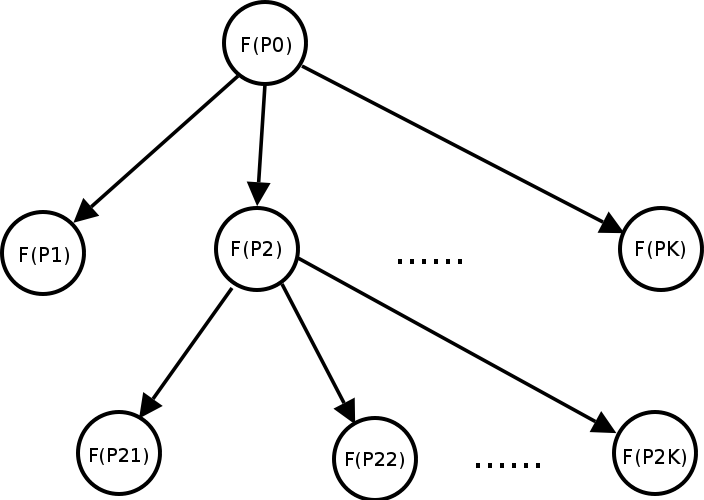
\includegraphics[scale=0.7]{images/02_00_Branch_and_Bound.png}
    \caption{Esempio di albero associato all'esecuzione dell'algoritmo}
\end{figure}

E' inoltre importante tenere a mente che:

\begin{remark}[EFFICIENZA DELL'ALGORITMO]
    L'efficienza dell'algoritmo è \textbf{fortemente influenzata} da:
    \begin{enumerate}
        \item \textbf{Partizionamento del problema} nelle sue restrizioni.
        \item \textbf{Scelta dei rilassamenti} associati alle restrizioni (bisogna
            generare \textit{problemi semplici da risolvere}, ma che contrinuiscano
            con \textit{lower bound ragionevoli}).
    \end{enumerate}
\end{remark}

Infine, ricollegandoci a quanto detto sopra sugli algoritmi di ricerca ad albero al
caso peggiore, sottolineaiamo che:

\begin{remark}
    Branch and Bound è un \textit{algoritmo di enumerazione implicita} perché si comporta 
    esattamente come un \textit{algoritmo di enumerazione} (cioè "prova" tutte le soluzioni 
    possibili fino a trovare quella ottima), ma ne \textbf{scarta alcune} dimostrando 
    a priori la loro \textit{non ottimalità}.
\end{remark}
